\renewcommand*{\arraystretch}{1.1}

\noindent\begin{tabularx}{17cm}{|p{1.95cm}|X|}
	\hline
	number      & 10                                                          \\ \hline
%
	title       & Central Person for a Tag                                                           \\ \hline
	\multicolumn{2}{|c|}{ 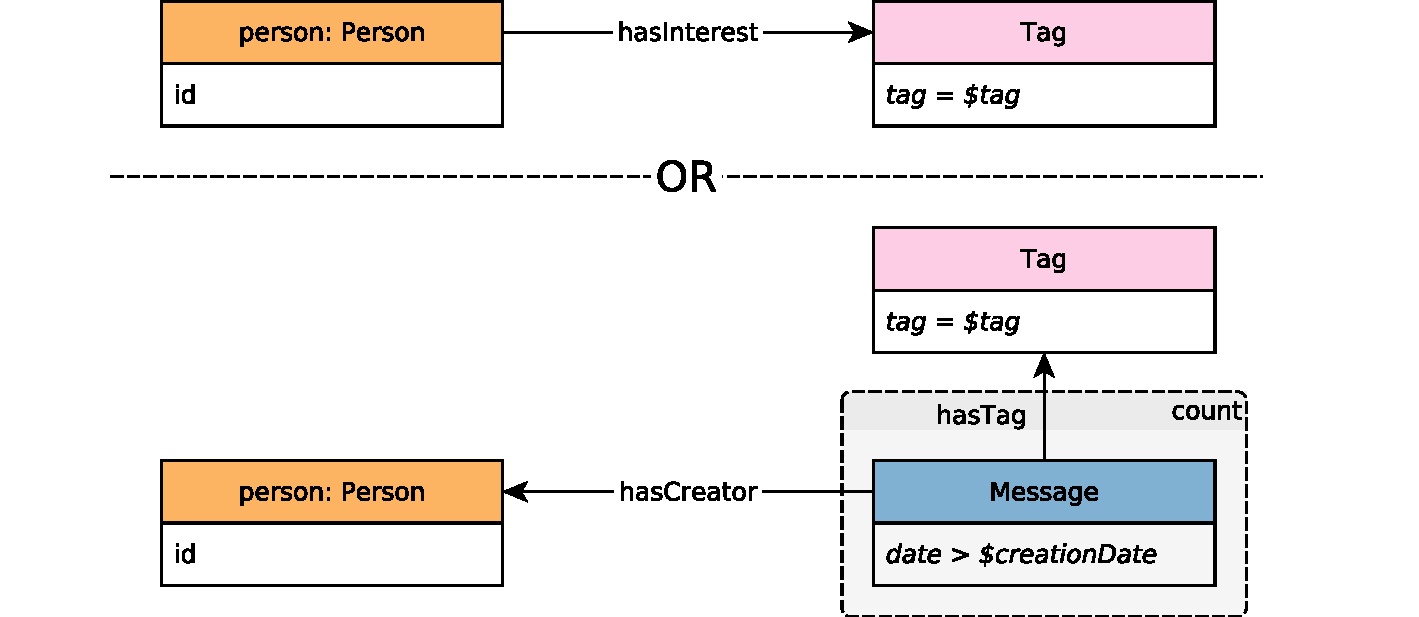
\includegraphics[scale=\patternscale,margin=0cm .2cm]{patterns/q10}} \\ \hline
	description & Given a Tag, find all Persons that are either interested in the Tag, or
have written a Message (Post or Comment) with creation date after a
given date and that has a given Tag. For each Person, compute the score
as the sum of the following two aspects:

\begin{itemize}
\tightlist
\item
  100, if the Person has this tag as their interest, or 0 otherwise
\item
  number of messages by this person with the given tag
\end{itemize}
 \\ \hline
	
%
	parameters  &
	\vspace{1.1ex}{\begin{tabularx}{14.2cm}{|c|l|m{2cm}|Y|} \hline
	\cellcolor{black!70} \color{white} $\mathsf{1}$ & \varname{tag} & \cellcolor{gray!20} \vartype{32bitInteger} &  \\\hline
	\cellcolor{black!70} \color{white} $\mathsf{2}$ & \varname{date} & \cellcolor{gray!20} \vartype{Date} &  \\
	\end{tabularx}} \\ \hline
%
	result      &
	\vspace{1.1ex}{\begin{tabularx}{14.2cm}{|c|l|m{2cm}|Y|} \hline
	\cellcolor{black!70} \color{white} $\mathsf{1}$ & \varname{person.id} & \cellcolor{gray!20} \vartype{64bitInteger} &  \\\hline
	\cellcolor{black!70} \color{white} $\mathsf{2}$ & \varname{score} & \cellcolor{gray!20} \vartype{32bitInteger} &  \\\hline
	\cellcolor{black!70} \color{white} $\mathsf{3}$ & \varname{friendsScore} & \cellcolor{gray!20} \vartype{32bitInteger} & The sum of the score of the Person's friends \\
	\end{tabularx}} \\ \hline
	%
	sort        &
	\vspace{1.1ex}{\begin{tabular}{|c|l|c|} \hline
	\cellcolor{black!70} \color{white} $\mathsf{1}$ & \varname{score + friendsScore} & \cellcolor{gray!20} $\desc$ \\\hline
	\cellcolor{black!70} \color{white} $\mathsf{2}$ & \varname{person.id} & \cellcolor{gray!20} $\asc$ \\
	\end{tabular}} \\ \hline
	%
	limit       & 100 \\ \hline
	%
	choke points &
	\multicolumn{1}{>{\raggedright}X|}{
		\chokepoint{1.2}, 
		\chokepoint{2.1}, 
		\chokepoint{2.3}, 
		\chokepoint{3.2}
		}\\ \hline
\end{tabularx}
\clearpage